% %%%%%%%%%%%%%%%%%%%%%%%%
% CU Big Data Class
% with Greg Greenstreet
% 23 April 2014
% Scott Hendrickson
% @DrSkippy27
% Gnip
% %%%%%%%%%%%%%%%%%%%%%%%%

\documentclass{beamer}
\setbeamertemplate{navigation symbols}{}

% THEMES
\usetheme{gnip}
% PACKAGES
\usepackage[group-separator={,}]{siunitx}
%\usepackage{fontspec}
\usepackage{graphicx}
\usepackage{tikz}
% see http://texblog.org/2008/05/07/fwd-equal-cell-width-right-and-centre-aligned-content/
\newcolumntype{x}[1]{%
>{\centering\hspace{0pt}}p{#1}}%
% FOOTER
\setbeamertemplate{footline}[text line]{
\colorbox{white}{\parbox[22px]{\paperwidth} {\color{linecolour} {\line(1,0){500} \\ \hfill @DrSkippy27 @gnip}}}
}
\beamersetuncovermixins{\opaqueness<1>{25}}{\opaqueness<2->{15}}

\usepackage{minted}
\usepackage{tikz}

\begin{document}
\title{Social Data Science}
\author{Scott Hendrickson \\ Principal Data Scientist, Gnip \\  @DrSkippy27}
\date{\today} 

% title

\begin{frame}
\titlepage
\end{frame}

%%%%%%%%
\section{Social Data}
{
\usebackgroundtemplate{\includegraphics[width=4cm]{./imgs/ink.jpg}}
\begin{frame}
\textcolor{black} {
\hfill \Huge \insertsection}
\end{frame}
}


% Feels like this
\begin{frame}
  \begin{center}
    \includegraphics[height=6.2cm]{./imgs/wheredoessocialdatacomefrom.jpg}
  \end{center}
\end{frame}

\begin{frame}\frametitle{Common Social Data Sources}
{\Huge
\begin{itemize}
\item APIs
\item scraping
\item firehose
\end{itemize}
}
\end{frame}

% Firehoses

\begin{frame}\frametitle{Firehose}
\begin{center}
{\Huge Continuous stream \\ [8pt] of activities \\ [15pt] in near-real time}
\end{center}
\end{frame}

% Volumes

\begin{frame} \frametitle{Firehose volumes}
\begin{table}
\begin{tabular}{l|r}
\hline
   {Publisher}   &   {Daily Activity}   \\
\hline 
    Twitter      &      520M   \\
    Tumblr      &       110M   \\
    Foursquare &       4.2M \\
    Wordpress Posts &     1M   \\
    Wordpress Comments & 1.7M \\
    Disqus       &       1.9M  \\
    Engagement (likes, votes) & >60M  \\
\hline
\end{tabular}
\end{table}
\end{frame}

%
\begin{frame}\frametitle{Every day @Gnip}
\begin{center}
{\Huge $\frac{3}{4}$ Billion IN \\ [18pt] 4 Billion + OUT}
\end{center}
\end{frame}

%%%%%%%%

\section{Data Science}
{
\usebackgroundtemplate{\includegraphics[width=5cm]{./imgs/ink.jpg}}
\begin{frame}
\textcolor{black} {
\hfill \Huge \insertsection}
\end{frame}
}

\begin{frame}
  \begin{center}
    \includegraphics[width=9.5cm]{./imgs/conway_datascientist.png} \\
    \textcolor{white}{\tiny \url{https://s3.amazonaws.com/aws.drewconway.com/latexviz/venn_diagram/data_science.html}}
  \end{center}
\end{frame}

\begin{frame}\frametitle{Social Data Processing Pipeline}
  \begin{center}
    \includegraphics[width=11cm]{./imgs/pipeline.png} \\
  \end{center}
\end{frame}

\begin{frame}\frametitle{Three Kinds of Research Projects}
\begin{center}
{\Large 
\begin{enumerate}
\item Descriptive
	\begin{itemize}
	\item Provides systematic information about a social data set
	\item May not begin with hypotheses, but to develop one as you go
	\item Detect anomalies
	\end{itemize}
\item Exploration
	\begin{itemize}
	\item Explores a social phenomena
	\item Provides background information needed to plan descriptive or explanatory research
	\item Trial and error or hypothesis driven
	\end{itemize}
\item Explanation
	\begin{itemize}
	\item 3 Levels: Relationship, Models, Prediction
	\item Ideas about the possible causes of a social phenomenon
	\item Plan a study that can provide systematic evidence for/against ideas about cause
	\end{itemize}
\end{enumerate}
}
\end{center}
\end{frame}

\begin{frame}\frametitle{Data Exploration}
  \begin{center}
    \includegraphics[height=7cm]{./imgs/exploration.png} \\
  \end{center}
      \textcolor{white}{\tiny \url{http://saedsayad.com/data_mining_map.htm}}
\end{frame}

\begin{frame}\frametitle{Data Modeling}
  \begin{center}
    \includegraphics[width=5.8cm]{./imgs/modeling.png} \\
  \end{center}
      \textcolor{white}{\tiny \url{http://saedsayad.com/data_mining_map.htm}}
\end{frame}

\begin{frame}\frametitle{Fundamental Processes}
	\begin{enumerate}
	\item Networks - e.g. 6-degrees, percolation
	\item Agent models
	\item Time series - e.g. ``Social Media Pulse''
	\end{enumerate}
\end{frame}
%%%%%%%%

\section{Time Series: Social Media Pulse}
{
\usebackgroundtemplate{\includegraphics[width=5.5cm]{./imgs/ink.jpg}}
\begin{frame}
\textcolor{black} {
\hfill \Huge \insertsection}
\end{frame}
}

\begin{frame}\frametitle{Simple Mention Counts}
  \begin{center}
    \includegraphics[width=8cm]{./imgs/TOY_bars.pdf} \\
  \end{center}
\end{frame}

\begin{frame}\frametitle{Unexpected: earthquake}
  \begin{center}
    \includegraphics[width=11cm]{./imgs/SMP_va_quake.pdf}
  \end{center}
\end{frame}

% Buckets and Sampling

\begin{frame}
\frametitle{Mentions and time series} 
We start by bucketing our mention counts by time periods, the activity rate is:
\begin{equation*}
    \label{eq:rateEst}
    \bar{r} = \frac{N}{T},
\end{equation*}
General model for activity rates:
\begin{equation*}
    \label{eq:tbe}
    p_{activity}(t) = r e^{-r t}.
\end{equation*}
give Poisson distribution:
\begin{equation*}
    \label{eq:poisson}
    P(n) = \frac{e^{-r t} (r t)^n}{n!}.
\end{equation*}
\end{frame}

\begin{frame}
\frametitle{Confidence intervals} 
Confidence intervals for the Poisson distribution with confidence level equal to $100\%(1-\alpha)$ 
are given by,
\begin{equation}
    \label{eq:chisqconf}
    \frac{1}{2T} \chi^2(\alpha/2;2n) \leq r \leq \frac{1}{2T} \chi^2(1-\alpha/2;2n+2)
\end{equation}
where $\chi^2$ is the inverse cumulative distribution function, $CDF^{-1}(p; n)$, of the $\chi^2$ 
distribution.
\end{frame}

\begin{frame}
\frametitle{90\% confidence intervals?} 
%%%%%
% table: poisson intervals
%
\begin{table}[!h]\centering
    \begin{tabular}{r|x{3.5cm}|c|c}
     \hline
$n$ & Interval Bounds & Interval Size ($\delta n$) & Relative Interval\\ 
\hline 
1 &   0.0513, 4.744  & 4.693 & 4.693\tabularnewline 
2 &   0.3554, 6.296  & 5.940 & 2.970\tabularnewline 
3 &   0.8177, 7.754  & 6.936 & 2.312\tabularnewline 
4 &   1.366, 9.154  & 7.787 & 1.947\tabularnewline 
5 &   1.970, 10.51  & 8.543 & 1.709\tabularnewline 
10 &   5.426, 16.96  & 11.54 & 1.154\tabularnewline 
30 &  21.59, 40.69  & 19.10 & 0.6366\tabularnewline 
40 &  30.20, 52.07  & 21.87 & 0.5468\tabularnewline 
50 &  38.96, 63.29  & 24.32 & 0.4864\tabularnewline 
500 &  463.8, 538.4  & 74.58 & 0.1492\tabularnewline 
750 &  705.5, 796.6  & 91.11 & 0.1215\tabularnewline 
1000 &  948.6,  1054.  & 105.0 & 0.1050\tabularnewline 
\end{tabular}
\end{table}
%
%%%%%
\end{frame}


\begin{frame}\frametitle{Make the buckets bigger?}
  \begin{center}
    \includegraphics[width=8cm]{./imgs/fig2.pdf}
  \end{center}
\end{frame}


\begin{frame}\frametitle{Ignore smaller signals?}
  \begin{center}
    \includegraphics[width=7cm]{./imgs/fig3a.pdf} \\
    \includegraphics[width=7cm]{./imgs/fig3b.pdf} 
  \end{center}
\end{frame}


\begin{frame}
  \begin{center}
\begin{figure}[!b]
\begin{center}
% http://cremeronline.com/LaTeX/minimaltikz.pdf
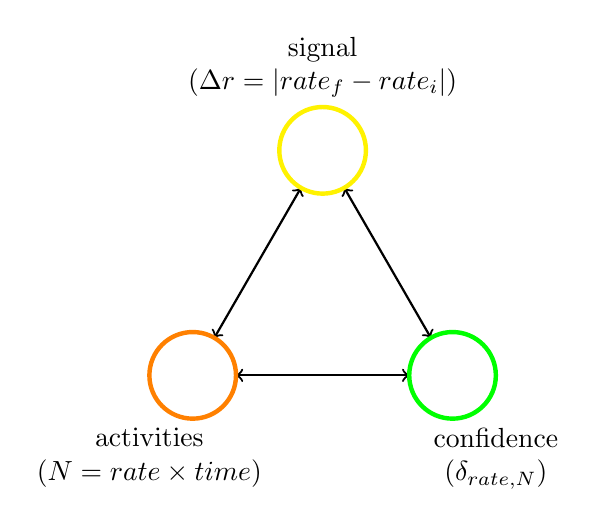
\begin{tikzpicture}[scale=1.1]]
% arrows
\draw [thick, <->] (0.25000000000000006, 0.4330127018922193) -- (1.25, 2.165063509461097) ;
\draw [thick, <->] (1.75, 2.165063509461097) -- (2.75, 0.4330127018922193) ;
\draw [thick, <->] (2.5, 0) -- (0.5, 0) ;
% circles
\draw [orange, ultra thick] (0,0) circle [radius=0.5];
\draw [yellow, ultra thick] (1.5,2.598) circle [radius=0.5];
\draw [green, ultra thick] (3,0) circle [radius=0.5];
% labels
\node[align=center, below] at (-0.5,-0.5){activities\\($N=rate \times time$)};
\node[align=center, above] at (1.5,3.098){signal\\($\Delta r=|rate_f-rate_i|$)};
\node[align=center, below] at (3.5,-0.5){confidence\\($\delta_{rate,N}$)};
\end{tikzpicture}
\end{center}
\end{figure}
  \end{center}
\end{frame}

% Events
\begin{frame}\frametitle{Unexpected: earthquake}
  \begin{center}
    \includegraphics[width=11cm]{./imgs/SMP_va_quake.pdf}
  \end{center}
\end{frame}

\begin{frame}\frametitle{Classifying events}
\begin{table}
\begin{tabular}{ m{2cm} | m{ 2.5cm} | m{4cm}}
\hline
Type & Response & Examples \\ \hline
Expected    &  Build-up/Decay & Hurricane Sandy \newline Olympics \\ \hline
Unexpected (many obs.) & Social Media \newline Pulse & Beyonc\'{e} VMAs \newline  Mexico earthquake \newline  Steve Jobs \\ \hline
Unexpected  (network spread) & Network \newline Models  & Osama bin Laden \newline  Whitney Houston \newline  Syrian dissidents \\ \hline
\end{tabular}
\end{table}
\end{frame}

% Model

\begin{frame}
\frametitle{Social media pulse} 
Given an event, the probability of an activity from one person,

\begin{equation*}
f(t) = \lambda \exp(-\lambda (t-t_0)), \text{ for } t \geq 0.
\end{equation*}

Many people posting on same cue; so sum of random variables 

\begin{equation*}
S = X_1 + X_2 + \ldots + X_{n \text{ posters}}
\end{equation*}

Gamma probability distribution function,

\begin{equation*}
f_S(t) = \frac{ \beta^{-\alpha} (t-t_0)^{\alpha-1} \exp( \frac{-(t-t_0)}{\beta}) } {\Gamma(\alpha)}
\end{equation*}

Cumulative distribution is the ``generalized regularized incomplete gamma function'',

\begin{equation*}
F_S(t) = Q(\alpha, 0, \frac{ (t-t_0)}{\beta})
\end{equation*}
\end{frame}

% gamma plots

\begin{frame}
  \begin{center}
   \includegraphics[height=6cm]{./imgs/SMP_gammadist.pdf}
  \end{center}
\end{frame}

\begin{frame}\frametitle{Why model half-life?}
{\Large
\begin{itemize}
\item predict total story volume
\item compare half-lives
\item anomalous story evolution
\end{itemize}
}
\end{frame}

\begin{frame}
  \begin{center}
    \includegraphics[width=8cm]{./imgs/SMP_va_quake_fit1.pdf}
  \end{center}
\end{frame}

\begin{frame}
\frametitle{Compare events} 
We start with a least-squares fit of points up to the $2-3 \times$ time-to-peak.
\begin{equation*}
t_{time-to-peak} = \beta (\alpha - 1)
\label{eq:peak}
\end{equation*}
Average event response time,
\begin{equation*}
t_{avg} = \alpha \beta
\label{eq:avg}
\end{equation*}
Half-life (time to see half of the activities),
\begin{equation*}
t_{\frac{1}{2}life} = F^{-1}_S(\frac{1}{2}).
\label{eq:half}
\end{equation*} 
Story size,
\begin{equation}
F_S(t) = Q(\alpha, 0, \frac{ t-t_0}{\beta})
\label{incgamma}
\end{equation}
in terms of the incomplete gamma functions, 
\begin{equation}
S_{vol} = \int_0^\infty r(t) dt = N_{activities} F_S(t),
\label{eq:mass}
\end{equation}
\end{frame}

%%%%%%%%

\section{Topic Modeling -- Latent Semantic Indexing}
{
\usebackgroundtemplate{\includegraphics[width=4.5cm]{./imgs/ink.jpg}}
\begin{frame}
\textcolor{black} {
\hfill \Huge \insertsection}
\end{frame}
}

\begin{frame}
\begin{center}
{\Huge What do we talk about \\ [15pt] when they talk about X?} 
\end{center}
\hfill Apologies: Raymond Carver \\
\end{frame}

{
\usebackgroundtemplate{\includegraphics[width=\paperwidth]{./imgs/disqus_threads.png}}
\begin{frame}
\textcolor{black} {
\vfill \hfill \Large Disqus discussion threads}
\end{frame}
}

\begin{frame}\frametitle{Disqus Threads}
\begin{center}
{\Large 
\begin{enumerate}
\item 7 weeks of Disqus comments data
\item Key words: ``texting,'' ``driving'' and variants
\item Select top threads based on mentions
\item 61,406 comments from 365 threads
\end{enumerate}
}
\end{center}
\end{frame}

\begin{frame}\frametitle{Disqus Topic Model Approach}
\begin{center}
{\Large 
\begin{enumerate}
\item Find comments that mention key words
\item Corpus of comments (across many threads)
\item tf-idf matrix: terms $\times$ comments
\item LSI (rotate space to align with ``important'' dimensions, reduce dimensions)
\item K-means (quick-and-dirty clustering in reduced dimensional space)
\item \ldots rinse and repeat (looking for distinction and cohesion)
\end{enumerate}
}
\end{center}
\end{frame}

\begin{frame}
\frametitle{tf-idf and LSI in one page \dots} 
\begin{itemize}
\item tf: term frequency
\item: idf: inverse document frequency
\end{itemize}

LSI uses singular value decomposition to rotate  document matrix from tf-idf to reduce
dimensionality in a controlled way.

SVD lets us write the document matrix as,
\begin{equation*}
D = V\Sigma U^T
\label{eq:svd}
\end{equation*}
where $\Sigma$ is a diagonal matrix and the with values satisfying,
\begin{equation*}
\Sigma_{1,1} > \Sigma_{2,2} > \Sigma_{3,3} > \Sigma_{4,4} > \ldots
\label{eq:svd}
\end{equation*}

To reduce dimensions, truncate the $\Sigma$ matrix smallest values first.
\begin{equation*}
D^\prime \approx V\Sigma^\prime U^T
\label{eq:svd}
\end{equation*}
where $D^\prime$ has fewer columns according to how we trimmed $\Sigma$.
\end{frame}



\begin{frame}\frametitle{Disqus Topic Model}
\begin{center}
{\Large 
\begin{enumerate}
\item Same 7 weeks; same keywords
\item 32,856 comments from 16,886 threads
\item LSI: 500 features $\rightarrow$ 80 features
\item K-means: 80 clusters as topics (?!)
\end{enumerate}
}
\end{center}
\end{frame}

\begin{frame}
\begin{center}
{\Huge Focus on the intersection of \\[15 pt] Thread and Topic models}
\end{center}
\end{frame}

\begin{frame}\frametitle{Comments with key words over time}
  \begin{center}
    \includegraphics[width=9.5cm]{./imgs/time.pdf}
  \end{center}
\end{frame}

\begin{frame}\frametitle{Disqus Thread Activity over Time}
  \begin{center}
    \includegraphics[width=9.5cm]{./imgs/timebythread.pdf}
  \end{center}
\end{frame}

\begin{frame}\frametitle{Disqus Topics Activity over Time}
  \begin{center}
    \includegraphics[width=9.5cm]{./imgs/timebycluster.pdf}
  \end{center}
\end{frame}

\begin{frame}\frametitle{Dominant Topics $\times$ Threads?}
  \begin{center}
    \includegraphics[width=9.5cm]{./imgs/gg_heat.pdf}
  \end{center}
\end{frame}

\begin{frame}\frametitle{When we talk about texting and driving, we talk about \ldots}
\begin{center}
{\Large 
\begin{enumerate}
\item Topic 12: poor graphic design
\item Topic 50: fake ids and fake drivers licenses
\item Topic 58: health/accident insurance
\item Topic 62: drunk drivers
\item Topic 64: buses and bus drivers
\item Topic 67: bikes, bike lanes
\item Topic 68: trucks and truck drivers
\end{enumerate}
}
\end{center}
\end{frame}

\begin{frame}
  \begin{center}
    {\Large Thank you!}  \\ [20pt]
    \includegraphics[width=3cm]{./imgs/logo.png} \\ [15pt]
    \begin{itemize}
    \item Presentation, data, vis. code at: \url{http://github.com/DrSkippy27/Disqus-Lightening-2013}
    \end{itemize}
  \end{center}
\end{frame}

\end{document}
